\chapter{Day and Night: The Sun}\label{ch:g1:day-and-night}

Every morning the Sun comes back, as if it had never left. It climbs,
slides down the other side of the sky, disappears --- and the street
lamps take over. Day, night, day, night: the oldest rhythm in the
world. Where does the Sun go at night? Let us follow it.

\section{The Sun's journey}

\begin{example}[One day of Sun]\label{ex:g1:day-and-night:journey}
Watch the Sun's place in the sky through one day (sideways, never
straight at it!). In the morning it sits low, near the rooftops, on
one side of the sky. Through the morning it climbs. At midday it
stands at its highest. In the afternoon it comes down on the
\emph{other} side, and in the evening it slips below the rooftops
there. The side where it rises in the morning is always the same ---
tomorrow it will rise there again.
\end{example}

\begin{omfigure}
\begin{tikzpicture}[scale=0.85]
  \draw[thick] (0,0) -- (11,0);
  \draw[dashed, omExo] (1.2,0.4) .. controls (3.5,3.4) and (7.5,3.4)
    .. (9.8,0.4);
  \fill[omThm] (1.6,0.85) circle (0.35);
  \fill[omThm] (5.5,2.65) circle (0.35);
  \fill[omThm] (9.4,0.85) circle (0.35);
  \node[below, font=\small] at (1.6,-0.15) {morning: it rises here};
  \node[above, font=\small] at (5.5,3.15) {midday: highest};
  \node[below, font=\small] at (9.4,-0.15) {evening: it sets here};
\end{tikzpicture}

{\small The Sun's daily road: up one side of the sky, over the top at
midday, down the other side. Tomorrow, the same road again.}
\end{omfigure}

\begin{omfigure}
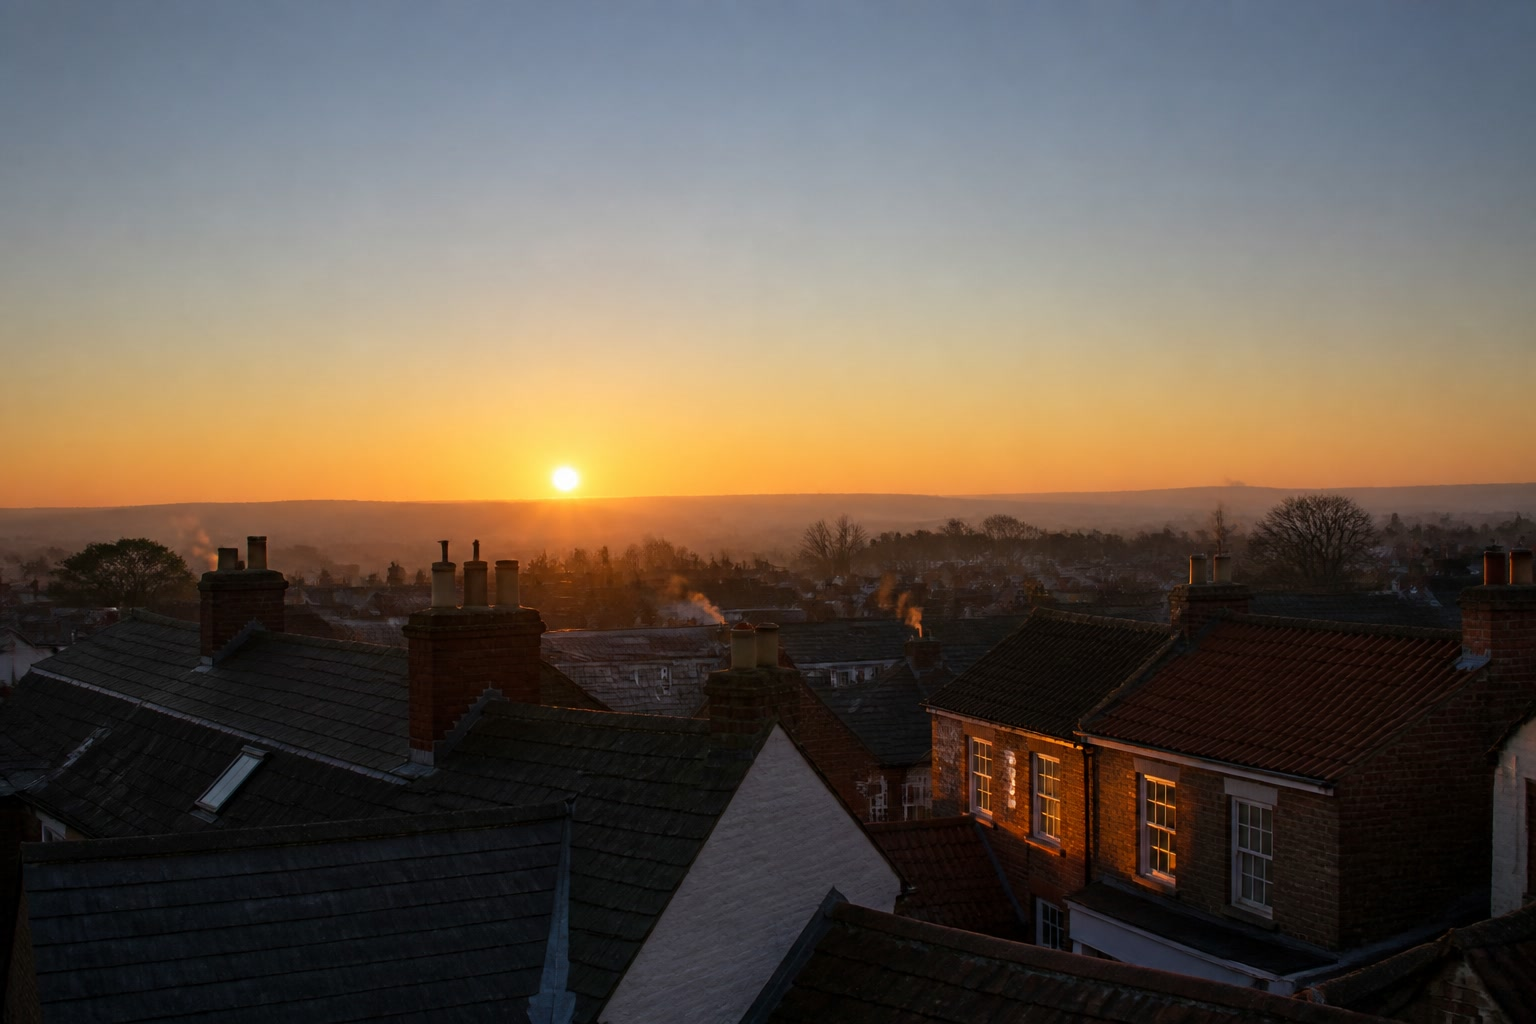
\includegraphics[width=0.6\linewidth]{images/book1/ai/g1-day-night-sunrise.jpg}

{\small \omterm{def:g1:day-and-night:daynight}{Sunrise}: the Sun appears over the rooftops, and the day begins.}
\end{omfigure}

\begin{definition}[Day and night]\label{def:g1:day-and-night:daynight}
\emph{Daytime}\index{daytime} is the part of the day when the Sun is
up in our sky, giving us \omterm{def:g1:light-and-shadows:source}{light}. \emph{Night}\index{night} is the part
when the Sun is gone from our sky and the world around us goes dark.
The moment the Sun appears is the \emph{sunrise}\index{sunrise}; the
moment it disappears is the \emph{sunset}\index{sunset}.
\end{definition}

\begin{remark}[The great lamp of the day]\label{rem:g1:day-and-night:lamp}
Remember the \omterm{def:g1:light-and-shadows:source}{light sources} of the last chapter: by day, the Sun is
the source that \omterm{def:g1:light-and-shadows:source}{lights} the whole world at once --- every street,
every playground, every sea. At night we make do with small sources:
lamps, torches, and the stars. That is why night is dark even though
the lamps are on: no small lamp can replace the great one.
\end{remark}

\begin{example}[The rhythm repeats]\label{ex:g1:day-and-night:rhythm}
Morning, midday, evening, night --- and then morning again. The
rhythm has never skipped once: after every night, a day; after
every day, a night. A whole turn of this wheel, one day \emph{and}
one night together, is what the calendar counts: Monday, Tuesday,
Wednesday, each is one turn of the wheel.
\end{example}

\section{Where does the Sun go at night?}

At night the Sun still shines --- but not on us. While we sleep, its
\omterm{def:g1:light-and-shadows:source}{light} falls on children on the other side of the world, who are
having their midday. The Sun does not go out; \emph{we} turn away
from it.

\begin{example}[The spinning Earth]\label{ex:g1:day-and-night:spinning}
The Earth --- the huge ball we all live on --- spins slowly, like a
merry-go-round, and we spin with it. When our side of the ball faces
the Sun, we have daytime. As the Earth keeps turning, our side slides
away from the sunlight into the dark: evening comes, then night. Keep
turning, and our side swings back into the \omterm{def:g1:light-and-shadows:source}{light}: \omterm{def:g1:day-and-night:daynight}{sunrise}! The Sun
only \emph{seems} to travel across our sky --- the real traveler is
the ground under our feet.
\end{example}

\begin{omfigure}
\begin{tikzpicture}[scale=0.85]
  \fill[omThm] (0.8,2.0) circle (0.5);
  \foreach \a in {0,30,...,330} {
    \draw[omThm] (0.8,2.0) ++(\a:0.7) -- ++(\a:0.3);
  }
  \node[below, font=\small] at (0.8,1.2) {Sun};
  \draw[thick] (7.0,2.0) circle (1.5);
  \begin{scope}
    \clip (7.0,2.0) circle (1.5);
    \fill[omExo, opacity=0.4] (7.0,0.4) rectangle (8.9,3.6);
  \end{scope}
  % the tilted spin axis, poking out of both poles
  \draw[thick, dash pattern=on 3pt off 2pt] (6.26,0.30) -- (7.74,3.70);
  % rotation arrow circling the axis near the north pole
  \begin{scope}[shift={(7.65,3.49)}, rotate=-23.5]
    \draw[-Stealth, thick, omDef]
      (-0.799,-0.082) arc (200:345:0.85 and 0.24);
  \end{scope}
  \fill[omDef] (5.62,2.5) circle (0.1);
  \node[left, font=\small] at (5.5,2.6) {here it is daytime};
  \fill[omDef] (8.38,2.5) circle (0.1);
  \node[right, font=\small] at (8.5,2.6) {here it is night};
  \node[font=\small, align=center] at (10.6,3.75)
    {the Earth turns\\around its tilted axis};
  \draw[omExo, very thin] (9.5,3.6) -- (8.55,3.3);
\end{tikzpicture}

{\small The Earth in the sunshine: the side facing the Sun has
daytime, the side turned away has night. The slow spin swaps them.}
\end{omfigure}

\begin{method}[Try it: be the Earth]\label{met:g1:day-and-night:beearth}
You need a lamp in a dark room, and yourself.
\begin{enumerate}
  \item The lamp is the Sun; your head is the Earth; your nose is
        your town.
  \item Face the lamp: \omterm{def:g1:light-and-shadows:source}{light} on your face --- your town has daytime.
  \item Turn slowly on the spot. The \omterm{def:g1:light-and-shadows:source}{light} slides off your cheek:
        that is evening.
  \item Back of your head to the lamp: your face is in the dark ---
        night in your town.
  \item Keep turning until the \omterm{def:g1:light-and-shadows:source}{light} returns to your cheek: \omterm{def:g1:day-and-night:daynight}{sunrise}!
\end{enumerate}
One full turn of you is one full day and night for your nose.
\end{method}

\begin{remark}[The Sun never switches off]\label{rem:g1:day-and-night:neveroff}
In the game of \cref{met:g1:day-and-night:beearth}, the lamp stayed
on the whole time --- only your turning made \omterm{def:g1:light-and-shadows:source}{light} and dark take
turns on your face. It is the same for the real Sun: it shines all
night long, on the other side of the world. Night is not the Sun
resting; it is our side of the ball looking the other way.
\end{remark}

\section{Exercises}

\begin{exercise}[$\star$]\label{exo:g1:day-and-night:1}
Put in order, starting from the morning: midday; \ \omterm{def:g1:day-and-night:daynight}{sunrise}; \ night;
\ \omterm{def:g1:day-and-night:daynight}{sunset}; \ afternoon.
\end{exercise}

\begin{exercise}[$\star$]\label{exo:g1:day-and-night:2}
Where is the Sun at midday: low near the rooftops, or at its highest
point? And your \omterm{def:g1:light-and-shadows:shadow}{shadow} at that moment --- long or short? (Think of
the last chapter.)
\end{exercise}

\begin{exercise}[$\star$]\label{exo:g1:day-and-night:3}
Does the Sun rise every morning on the same side of your house, or on
a different side each day? How could you check tomorrow?
\end{exercise}

\begin{exercise}[$\star$]\label{exo:g1:day-and-night:4}
True or not true: ``At night, the Sun switches off.'' Explain your
answer with \cref{rem:g1:day-and-night:neveroff}.
\end{exercise}

\begin{exercise}[$\star$]\label{exo:g1:day-and-night:5}
While you are having breakfast in the morning \omterm{def:g1:light-and-shadows:source}{light}, what are
children on the opposite side of the Earth most likely doing?
\end{exercise}

\begin{exercise}[$\star$]\label{exo:g1:day-and-night:6}
Play \cref{met:g1:day-and-night:beearth} with a lamp. When the \omterm{def:g1:light-and-shadows:source}{light}
shines on your right cheek and you keep turning the same way, what
comes next for your nose: \omterm{def:g1:day-and-night:daynight}{sunrise} or \omterm{def:g1:day-and-night:daynight}{sunset}?
\end{exercise}

\begin{exercise}[$\star$]\label{exo:g1:day-and-night:7}
Which is the real traveler, the Sun across our sky or the ground
under our feet? Say it in your own words.
\end{exercise}

\begin{exercise}[$\star$]\label{exo:g1:day-and-night:8}
Count with the calendar: how many \omterm{def:g1:day-and-night:daynight}{sunrises} are there in one week?
How many nights?
\end{exercise}

\begin{exercise}[$\star\star$]\label{exo:g1:day-and-night:9}
Zoe says: ``If the Earth stopped turning, our town would keep daytime
forever.'' Could she be right --- and what would children on the
other side of the Earth say about her idea?
\end{exercise}
